\documentclass[serif,9pt]{beamer}
\usepackage{color,listings}
\usepackage{ragged2e}
\usepackage[spanish]{babel}
\usepackage[utf8]{inputenc}
\usepackage{graphicx}

\definecolor{dkgreen}{rgb}{0,0.6,0}
\definecolor{gray}{rgb}{0.5,0.5,0.5}
\definecolor{mauve}{rgb}{0.58,0,0.82}
\definecolor{lgray}{rgb}{0.99,0.97,0.95}
\newcommand{\X}{\textbf{X}}
\newcommand{\Y}{\textbf{Y}}
\newcommand{\Z}{\textbf{Z}}
\newcommand{\G}{\textbf{G}}
\newcommand{\R}{\textbf{R}}
\newcommand{\V}{\textbf{V}}
\newcommand{\Q}{\textbf{Q}}
\newcommand{\h}{\textbf{H}}
\newcommand{\T}{\textbf{T}}

\def\E{\mathbb{E}}
\def\C{\mathbb{C}}
\def\N{\mathbb{N}}

\setbeamercovered{transparent}


\usetheme{Frankfurt}
%\usecolortheme{rose}
%\usecolortheme{lily}
\usepackage{amsmath, multirow}
%\usepackage{color, amsmath, wrapfig, anysize, graphicx, hyperref, amsthm, fancyhdr, amssymb,geometry,amsfonts,float}

\newcommand{\ds}{\displaystyle}


\titlegraphic{
\includegraphics[width=4cm]{utfsm.eps}}%
   %\includegraphics[width=4cm]{fig/inria.eps}}

\begin{document}
\title{Una Arquitectura de Referencia para Web Browsers: Hacia una unificaci\'on de Conceptos de Seguridad} 
\author[Paulina Silva Ghio]{\textsc{Paulina Silva Ghio} \\ \medskip
\small{}
Departamento de Inform\'atica - UTFSM\\ \medskip
\url{pasilva@alumnos.inf.utfsm.cl}}
\institute[]{}
\date{24-11-2015.}

\begin{frame}[plain]
\titlepage
\end{frame}


\begin{frame}
\frametitle{Indice}
\tableofcontents
\end{frame} 


\section{Introducci\'on}
\subsection{Contexto}
\begin{frame}
\frametitle{Contexto}

	\begin{itemize}
		\item<1-> La guerra de los Navegadores: construir y parchar.
		\item<2-> El navegador web: herramienta de uso cotidiano.
		\item<3-> El usuario com\'un utiliza servicios.
		\item<4-> Distintos tipos, distintas implementaciones.
		\item<5-> Web 2.0 y 3.0: AJAX (Asynchronous Javascript and XML).
	\end{itemize}
\end{frame}


\begin{frame}
\frametitle{Browser en la Actualidad}
	\begin{figure}[h]
	    \centering
	    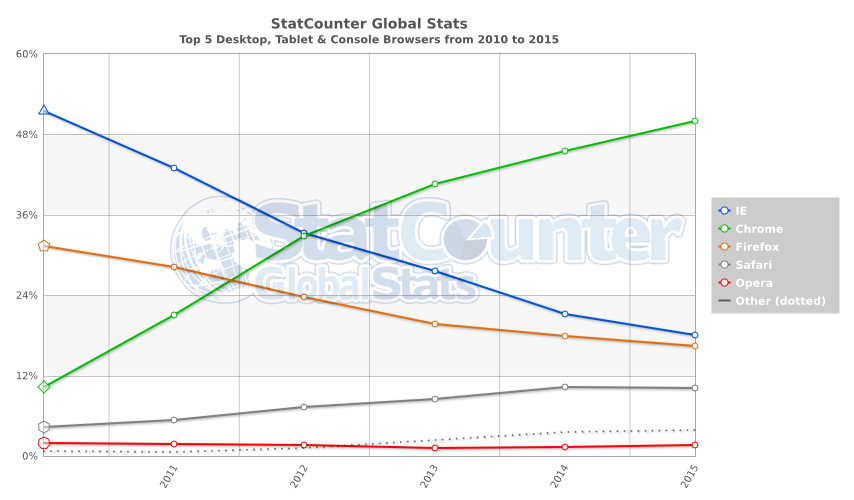
\includegraphics[width=1\textwidth]{figures/StatCounter-browser-ww-yearly-2010-2015.png}
	    \caption{Porcentaje de uso de Navegadores. Fuente: \cite{statBrow}}
	    \label{fig:UsageShare}
	\end{figure}
\end{frame}

\begin{frame}
	\frametitle{El Problema...}
	\begin{itemize}
		\item<1-> Sistemas actuales son muy complejos.
		\item<2-> Es necesario utilizar metodologías que aseguren: Requerimientos Funcionales y No-Funcionales.
		\item<3-> Defectos y errores en el Software generan vulnerabilidades.
		\item<4-> La Seguridad es un costo ``extra", a veces no considerado.
	\end{itemize}
	\begin{block}<5->{Las vulnerabilidades...}
		Ocurren por que no se ha tomado en cuenta la seguridad en el desarrollo.
	\end{block}
\end{frame}


\subsection{Seguridad...}
\begin{frame}
\frametitle{Seguridad...}
	\begin{block}<1->{Desde la perspectiva de seguridad \cite{WhyteHarrison}:}
		\begin{itemize}		
			\item<2-> ¿Qu\'e realizan las universidades o la industria?
			\item<3-> Proyectos de desarrollo de software, ¿cuanto se le dedica a la seguridad?
			\item<4-> ¿La industria asegura que los sistemas a construir, sean seguros?
		\end{itemize}
	\end{block}
	\begin{block}<5->{¿Qu\'e conceptos de seguridad sabe en promedio un estudiante graduado de carrera relacionada a Computer Science?}
		\begin{itemize}
			\item<6-> ¿La gente es autodidacta? o ¿aprende por necesidad?
			\item<7-> ¿La malla curricular es suficiente?
		\end{itemize}
	\end{block}
\end{frame}


\subsection{Desarrollo de Software y Seguridad}
\begin{frame}
\frametitle{Desarrollo de Software y Seguridad}
	\begin{itemize}
		\item<1-> ¿Qu\'e tanto se diferencian las preocupaciones del usuario com\'un y el desarrollador que crea los sistemas?
		\item<2-> ¿C\'omo desarrollar software seguro?
	\end{itemize}
	\begin{block}<3->{Construcci\'on de Software Seguro...}
		\begin{itemize}
			\item<4-> Los que participan en la construcci\'on: deben entender los problemas de seguridad.
			\item<5-> No basta saber como est\'a construido.
			\item<6-> Considerar la Seguridad desde el inicio del Proyecto.
			\item<7-> Seguridad como una Propiedad Sist\'emica.
		\end{itemize}
	\end{block}
\end{frame}


\subsection{Motivaci\'on para estudiar el Browser}
\begin{frame}
	\frametitle{Motivaci\'on para estudiar el Browser}
	\onslide<1->{El browser es una herramienta indispensable, \'este permite:}
	\begin{itemize}
		\item<2-> Nuevas formas de interactuar.
		\item<3-> Disminuir los costos de construir un programa Cliente (desde cero) para
el usuario del sistema.
		\item<4-> Seguridad (la que est\'a implementada en los Web Browser es bastante buena).
		\item<5-> Es una herramienta indispensable, por lo tanto el reuso es lógico.
	\end{itemize}
	
	\begin{block}<6->{Las preocupaciones principales}
	\begin{itemize}
		\item<7-> Los sistemas, a los que un usuario hace referencia, son llamados desde un Web Browser.
		\item<8-> Los stakeholders afectados: el usuario del Browser, el Host del usuario y hasta el Servicio extero usado.
		\item<9-> Falta de conocimientos de seguridad con respecto al Browser, podr\'ia afectar de forma directa el desarrollo de aplicaciones que lo utilizan y Stakeholders.
	\end{itemize}
	\end{block}
\end{frame}


\subsection{Contribuciones}
\begin{frame}
	\frametitle{Contribuciones}
	\begin{block}<1->{Objetivo General}
		\begin{itemize}
			\item<2-> Generar un cuerpo organizado de informaci\'on sobre el Web Browser y su seguridad.
			\item<3-> Sistematizar, organizar y clasificar el conocimiento adquirido en un documento, con formato semi-formal.Dado que hay conceptos poco claros y poca documentación formal.
			\item<4-> Para: profesionales como Estudiantes del \'area Inform\'atica que est\'en insertos en el \'area de Desarrollo de Software.
		\end{itemize}
	\end{block}
\end{frame}

\begin{frame}
	\frametitle{Contribuciones}
	\begin{block}<1->{Objetivos Espec\'ificos}
		\begin{itemize}
			\item<2-> Comprender los conceptos relacionados al navegador web, sus componentes, interacciones o formas de comunicaci\'on, amenazas y ataques a los que puede estar sometido, como tambi\'en los mecanismos de defensa. Esto se realizar\'a a trav\'es del desarrollo de un Estado del Arte sobre el Browser.
			\item<3-> Identificar actores, componentes, funciones, relaciones, requerimientos y restricciones del navegador, para lograr abstraer una Arquitectura de Referencia (AR) a partir de documentaci\'on disponible en Internet, blogs de desarrolladores, papers e iniciar un pequeño cat\'alogo de Patrones de Mal Uso. 
			\item<4-> Condensar el conocimiento obtenido en el punto anterior a trav\'es de documentos semi-formales.
			\item<5-> Una gu\'ia para comunicar los conceptos relevantes que pudieran afectar la relaci\'on existente entre un desarrollo de software y el navegador.
			\item<6-> Profundizar el conocimiento en ataques relacionados con m\'etodos de Ingenier\'ia Social.
		\end{itemize}
	\end{block}
\end{frame}

\begin{frame}
	\frametitle{Metodología basada en Fernandez \cite{braz2008eliciting,fernandez2013security}}
	\begin{block}<1->{Arquitectura de Referencia (AR)}
		\begin{itemize}
			\item<2-> Especifica la decomposici\'on del sistema en subsistemas, las interacciones entre estas partes y la distribuci\'on de funcionalidad entre ellas.
			\item<3-> Capturar la esencia de la arquitectura a trav\'es de una colecci\'on de sistemas similares, por medio del reuso arquitect\'onico
			\item<4-> Ayudar a los implementors o desarrolladores del software, a entender los trade-off cuando se diseñan nuevos sistemas
			\item<5-> Ayudar a los mantenedores de estos sistemas a entender el c\'odigo legacy usado.
			\item<6-> Comparar las diferencias en decisiones de diseño y poder entender los cambios realizados a lo largo del Desarrollo de un sistema.
			\item<7-> Mirada hol\'istica del Sistema.
		\end{itemize}
	\end{block}
	\begin{block}<8->{Patrones del Mal Uso}
		\onslide<9->{Permitir\'an enseñar y comunicar las posibles formas en que tal sistema puede ser usado inapropiadamente.}
	\end{block}
\end{frame}

\section{Marco Te\'orico de un Browser}
\begin{frame}
	\frametitle{Marco Te\'orico de un Browser}
	\begin{itemize}
		\item<1-> Arquitectura cliente/servidor
		\item<2-> Comunicaci\'on e Informaci\'on de estado: HTTP y canales.
		\item<3-> SSL/TLS
		\item<4-> HTML5 y XML (Markup Languages)
		\item<5-> CSS
		\item<6-> DOM
		\item<7-> Javascript (ECMAScript)
		\item<8-> Geolocalizaci\'on, WebWorkers y otros...
	\end{itemize}
	\begin{block}<9->{Desaf\'ios del navegador}
		\begin{itemize}
			\item<10-> Contenido y compatibilidad
			\item<11-> Navegaci\'on personalizada
			\item<12-> Navegaci\'on sin inconvenientes
			\item<13-> Seguridad
		\end{itemize}
	\end{block}
\end{frame}

\begin{frame}
	\frametitle{Arquitectura de Referencia (AR)}
	\begin{itemize}
		\item<1-> Describir los Stakeholders que interactuan con el sistema y que poseen preocupaciones/concerns de \'este.
		\item<2-> Patrones de Arquitectura.
		\item<3-> Atributos de calidad deseables que el sistema debe garantizar. Es importante solo destacar aquellos realmente necesarios, dado que un sistema sobrecargado con ellos tampoco es conveniente.
		\item<4-> Actualmente no hay un consenso de cómo definir una AR, lo que debería contener y cómo debería de construirse.
	\end{itemize}
	\begin{block}<5->{Ventajas}
		\begin{itemize}
			\item<6-> Comprender la estructura subyacente de un Web Browser y las interacciones que tendr\'a con otros sistemas.
			\item<7-> Proveer una base tecnol\'ogica modular y flexible. Al tener los subsistemas compartimentalizados es posible quitar y sacar piezas, que poseen interfaces similares, y de esa manera reusar lo otro sin tener que construir un sistema nuevo.
			\item<8-> Entrega una base para el desarrollo de otros Navegadores Web, sin explicar detalles de implementaci\'on.
		\end{itemize}
	\end{block}
\end{frame}

\section{(In)Seguridad en el Browser}
\begin{frame}
	\frametitle{Social Engineering Attacks o Ataques de Ingenier\'ia Social: Phishing}
	\begin{figure}[h]
        \centering
        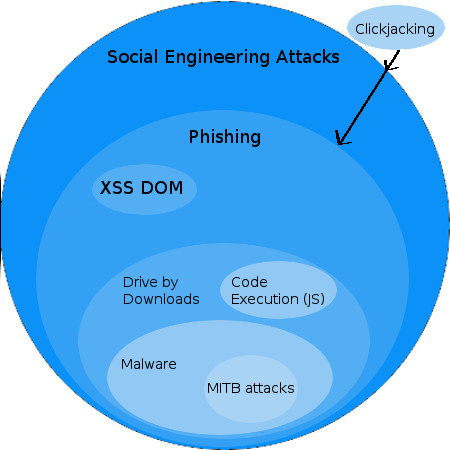
\includegraphics[scale=0.4]{figures/SEAttacks.jpg}
        \caption{Esquematizaci\'on de ataques de tipo Social Engineering.}
        \label{fig:SEattack}
    \end{figure}
\end{frame}

\begin{frame}
	\frametitle{Instalaci\'on de Malware o extensiones maliciosas}
	\begin{figure}[h]
        \centering
        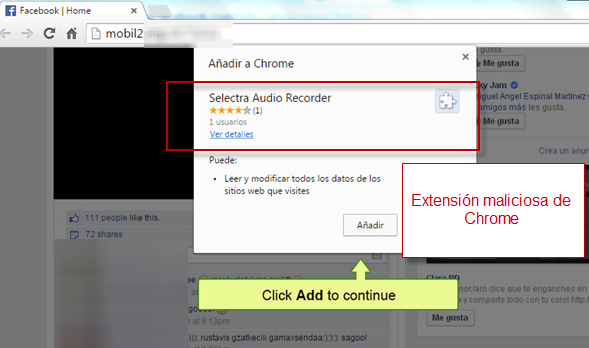
\includegraphics[scale=0.4]{figures/fbporn3.png}
        \caption{Fijarse en la barra de direcciones, para la p\'agina que supuestamente es Facebook.}
        \label{fig:Malware}
    \end{figure}
\end{frame}

\begin{frame}
	\frametitle{Extensiones Vulnerables}
	\begin{figure}[h]
        \centering
        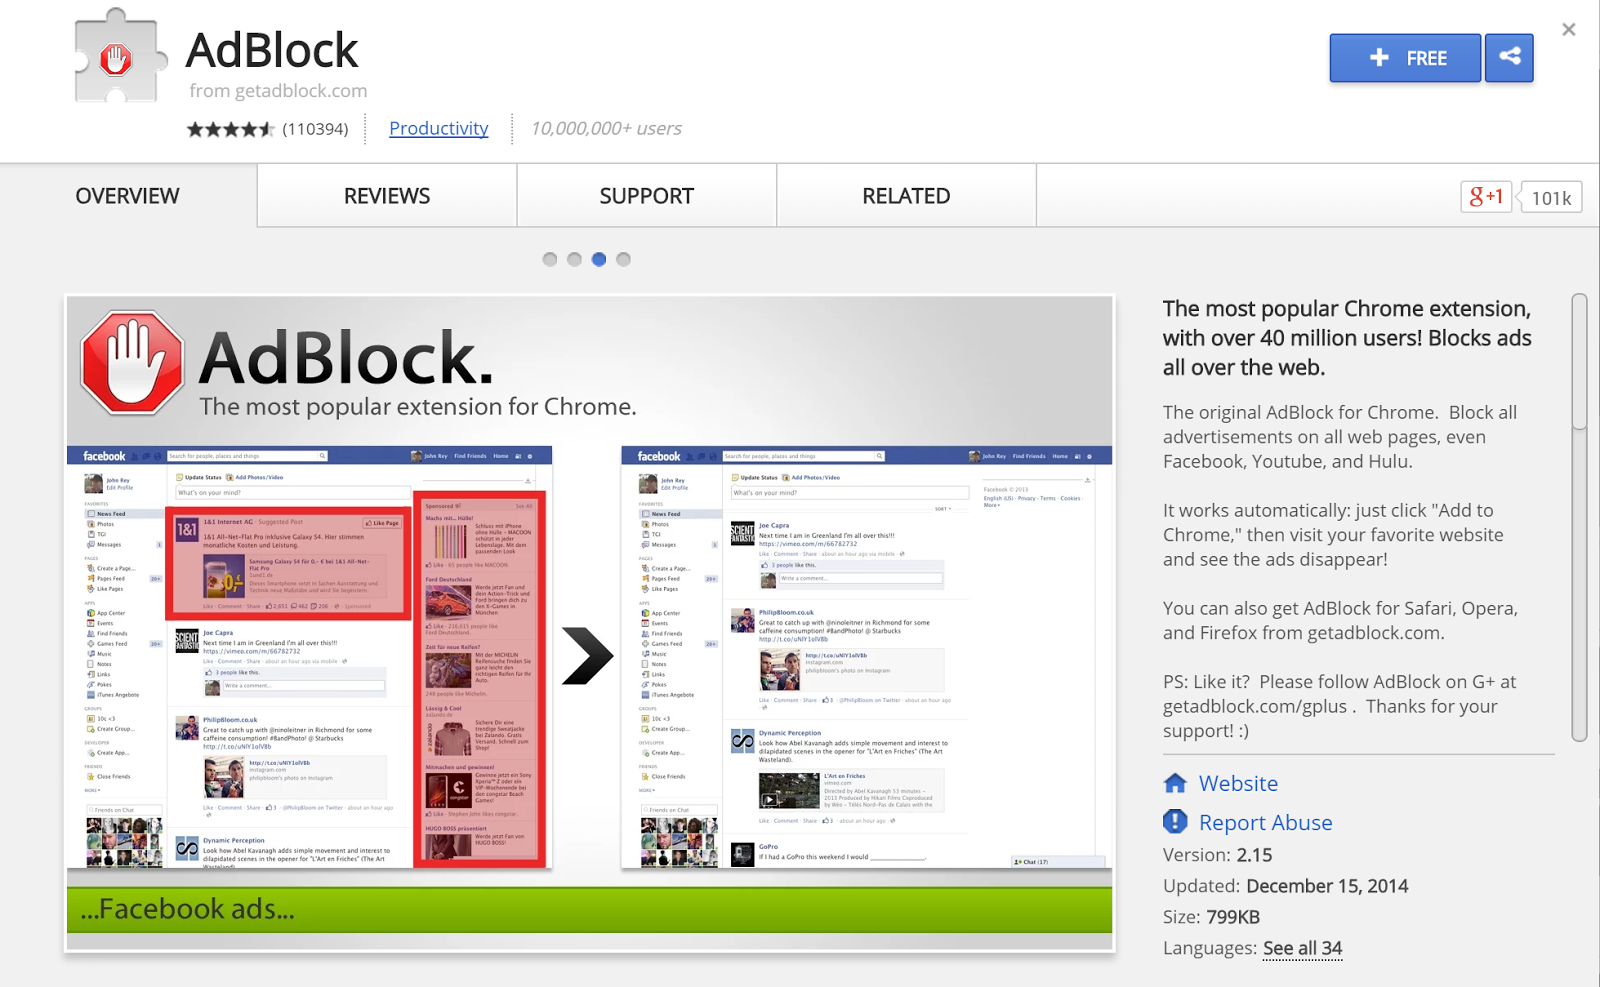
\includegraphics[scale=0.15]{figures/Adblock.png}
        \caption{¿Qu\'e suceder\'ia si una extensi\'on, confiable para los usuarios, permitiera generar ataques?}
        \label{fig:vulnExt}
    \end{figure}
\end{frame}

\begin{frame}
	\frametitle{Ejecuci\'on de c\'odigo Javascript y XSS-DOM}
		\begin{itemize}
			\item<1-> Ambos generan cambios en el DOM, pero de diferentes maneras (Uno es una especializaci\'on).
			\item<2-> La ejecuci\'on de javascript podr\'ia pasar ciertos controles de acceso (Javascript Capabilities).
			\item<3-> Puede terminar realizando conexiones con servidores maliciosos, sin que el usuario se de cuenta (XHR).
			\item<4-> El DOM puede ser modificado, de tal manera de engañar al usuario.
			\item<5-> XSS-DOM, el c\'odigo al lado del cliente se ejecuta de una manera distinta dada las modificaciones maliciosas que se han hecho al DOM.
		\end{itemize}
\end{frame}

\begin{frame}
	\frametitle{Man-in-the-Browser}
	\begin{figure}[h]
        \centering
        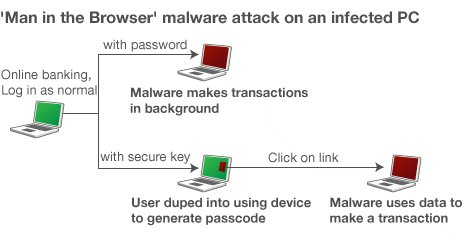
\includegraphics[scale=0.7]{figures/_58291188_malware_464v2.jpg}
        \caption{Normalmente el ataque se realiza cuando el usuario ha permitido la instalaci\'on en el Host de un ente malicioso: extensi\'on o programa}
        \label{fig:vulnExt}
    \end{figure}
\end{frame}

\subsection{Mecanismos de Defensa}
\begin{frame}
	\frametitle{Mecanismos de Defensa}
	\begin{itemize}
		\item<1-> SOP o Same Origin Policy
		\item<2-> CORS o Cross-Origin Resource Sharing
		\item<3-> HTTP Fields o Campos HTTP
		\item<4-> Sandboxing: Google Chrome/Chromium e Internet Explorer
		\item<5-> Aislaci\'on de Contenido
		\item<6-> Blacklist y Whitelist
		\item<7-> Sistema de Reputaci\'on
		\item<8-> Actualizaciones peri\'odicas en background
	\end{itemize}
\end{frame}


\section{Estado del Arte}
\begin{frame}
	\frametitle{Estado del Arte}
	\begin{itemize}
		\item<1-> No se encontr\'o informaci\'on actualizada sobre una Arquitectura de Referencia del Browser. Hay una \cite{preprint-grosskurth-browser-archevol}, pero es muy antigua.
		\item<2-> Poca documentaci\'on y no hay conceptos unificados.
	\end{itemize}
\end{frame}

\subsection{Google Chrome y Chromium}
\begin{frame}
	\frametitle{Google Chrome y Chromium}
	\begin{figure}[h]
	    \centering
	    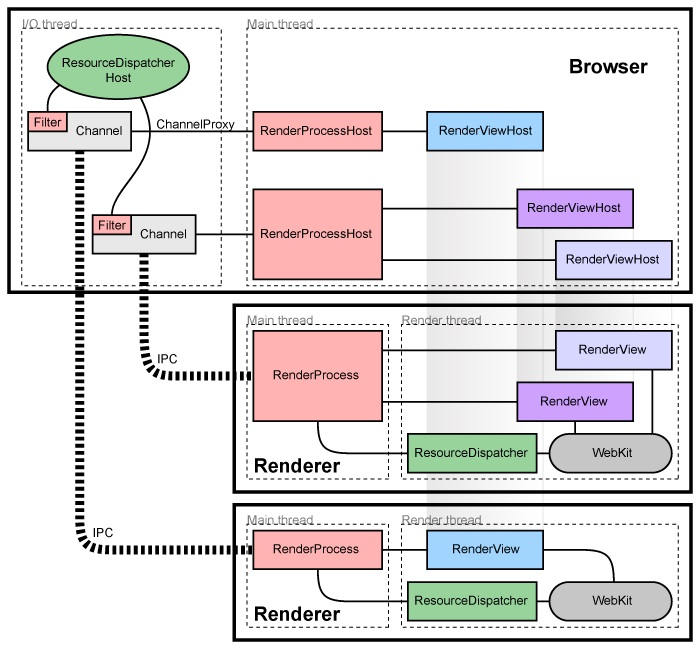
\includegraphics[scale=0.35]{figures/archGC.jpg}
	    \caption{Architectura Multiprocesos de Google Chrome. Fuente: \cite{multiProcGC}}
	    \label{fig:UsageShare}
	\end{figure}
\end{frame}

\begin{frame}
	\frametitle{Google Chrome y Chromium}
	\begin{figure}[h]
        \centering
        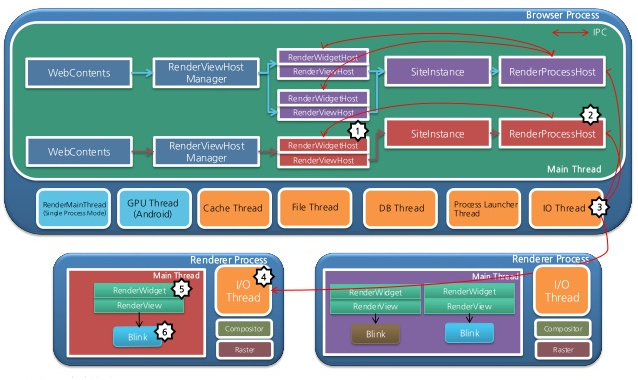
\includegraphics[scale=0.4]{figures/chromium-rendering-pipeline-28-638.jpg}
        \caption{Architectura de Chromium en detalle. Fuente: \cite{ChrRenderPipe}}
        \label{fig:archGC2}
    \end{figure}
\end{frame}

\subsection{Internet Explorer}
\begin{frame}
	\frametitle{Internet Explorer}
	\begin{figure}[h]
	    \centering
		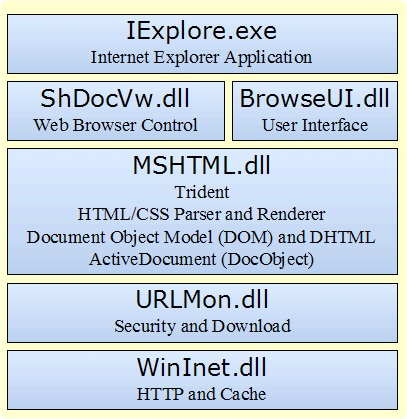
\includegraphics[scale=0.5]{figures/IEArch.jpg}
		\caption{Arquitectura de Internet Explorer. Fuente: \cite{IEArchImg}}
		\label{fig:archIE}
    \end{figure}
\end{frame}

\begin{frame}
	\frametitle{Internet Explorer}
	\begin{figure}[h]
        \centering
        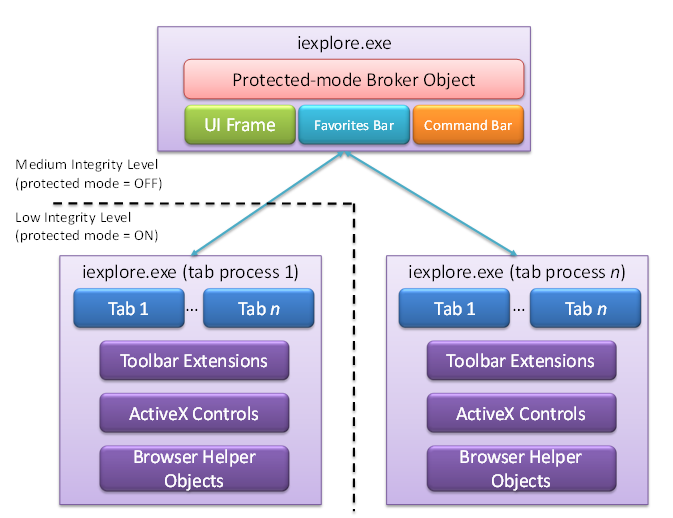
\includegraphics[scale=0.35]{figures/11_IE8andLooselyCoupledIELCIE_2.png}
        \caption{Arquitectura de Internet Explorer m\'as detallada. Fuente: \cite{IE8LCIE}}
        \label{fig:archIE2}
    \end{figure}
\end{frame}

\subsection{Firefox - Electrolysis}
\begin{frame}
	\frametitle{Firefox - Electrolysis}
	\begin{figure}[h]
        \centering
        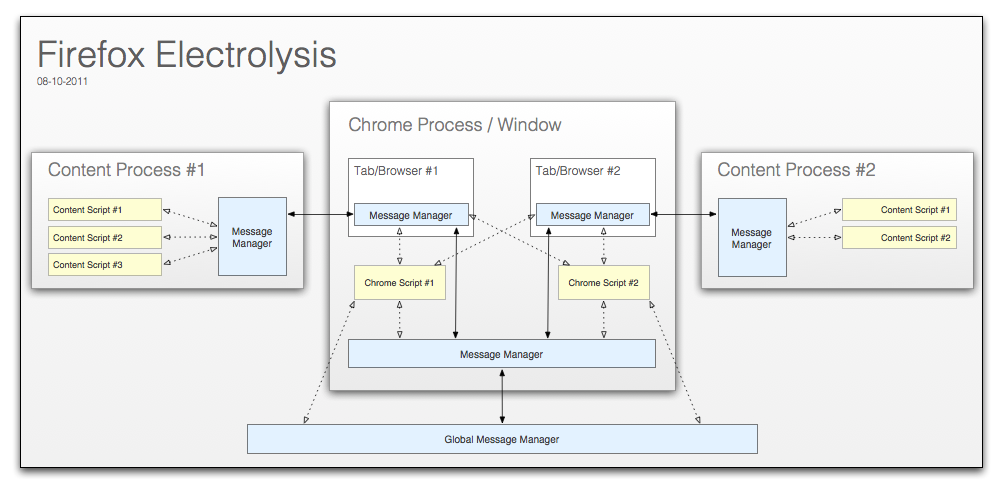
\includegraphics[scale=0.3]{figures/electrolysis.png}
        \caption{Firefox Electrolysis, Comunicaci\'on de procesos 1. Fuente: \cite{Firefox101}}
        \label{fig:ChromePComm1}
    \end{figure}
\end{frame}

\begin{frame}
	\frametitle{Firefox - Electrolysis}
	\begin{figure}[h]
        \centering
        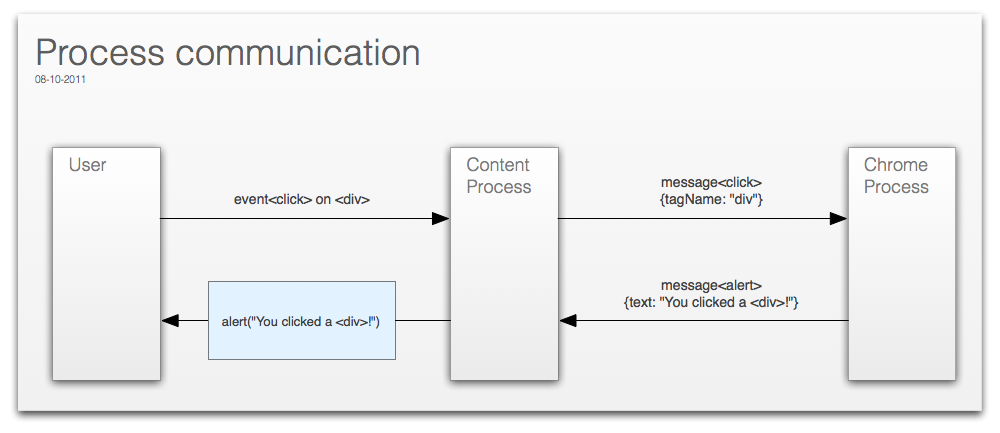
\includegraphics[width=1\textwidth]{figures/e10s-processes.png}
        \caption{Firefox Electrolysis, Comunicaci\'on de procesos 2. Fuente: \cite{Firefox101}}
        \label{fig:ChromePComm2}
    \end{figure}
\end{frame}

\section{Arquitectura de Referencia}
\begin{frame}
	\frametitle{Casos de Uso}
	\begin{figure}[h]
	    \centering
	    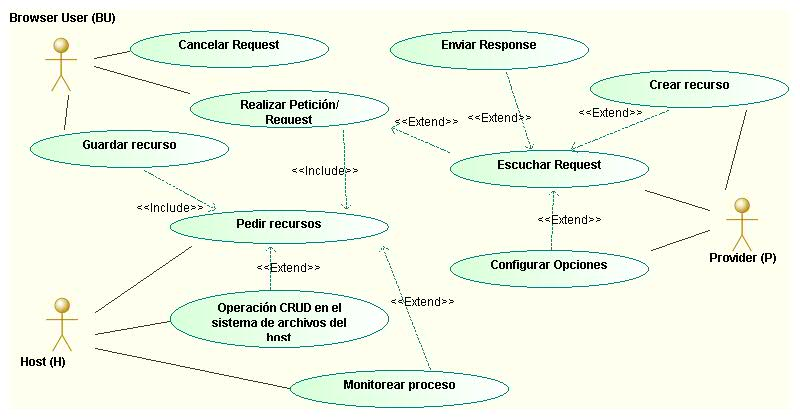
\includegraphics[scale=0.35]{figures/chap4/UCBrowser.jpg}
	    \caption{Diagrama de Caso de Uso del \textit{Web Browser}.}
	    \label{fig:CUBrowser}
	\end{figure}
\end{frame}

\begin{frame}
	\frametitle{Patr\'on Browser Infrastructure}
	\begin{figure}[h]
	    \centering
	    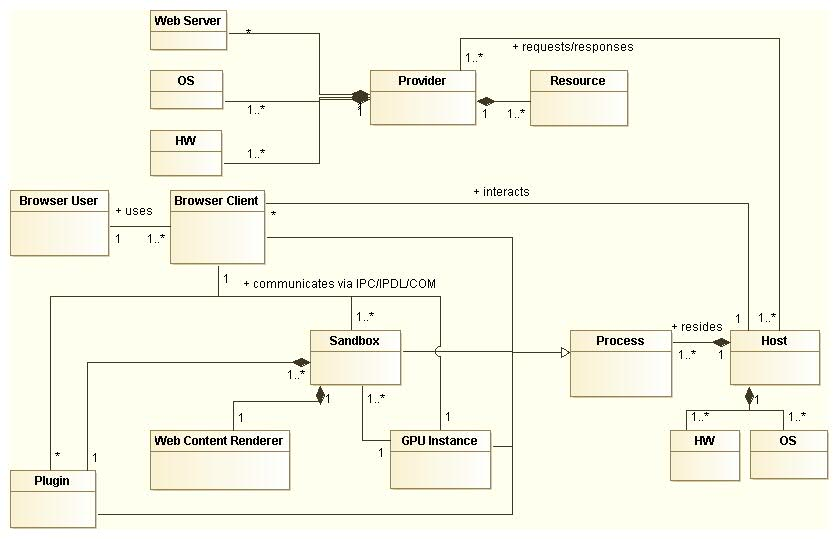
\includegraphics[scale=0.35]{figures/chap4/browserInfraPattern_v3.jpg}
	    \caption{Componentes de alto nivel del \textit{Browser}.}
	    \label{fig:BIPatt}
	\end{figure}
\end{frame}


\begin{frame}
	\frametitle{Din\'amica: Realizar Request}
	\begin{figure}[h]
	    \centering
	    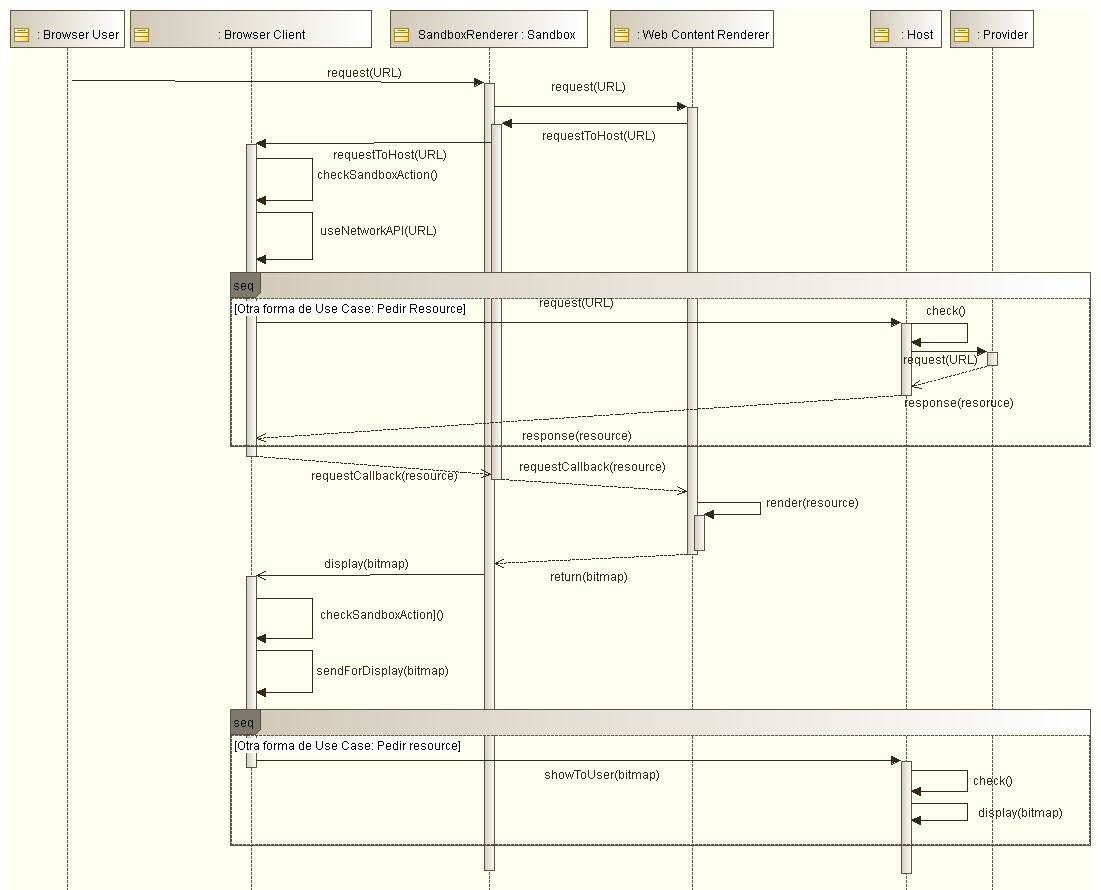
\includegraphics[scale=0.28]{figures/chap4/requestResource_v2.jpg}
	    \caption{Diagrama de Secuencia: Realizar Request.}
	    \label{fig:SecReq}
	\end{figure}
\end{frame}

\section{Patr\'on de Mal Uso}
\begin{frame}
	\frametitle{Diagrama de Actividad}
	\begin{figure}[h]
	    \centering
	    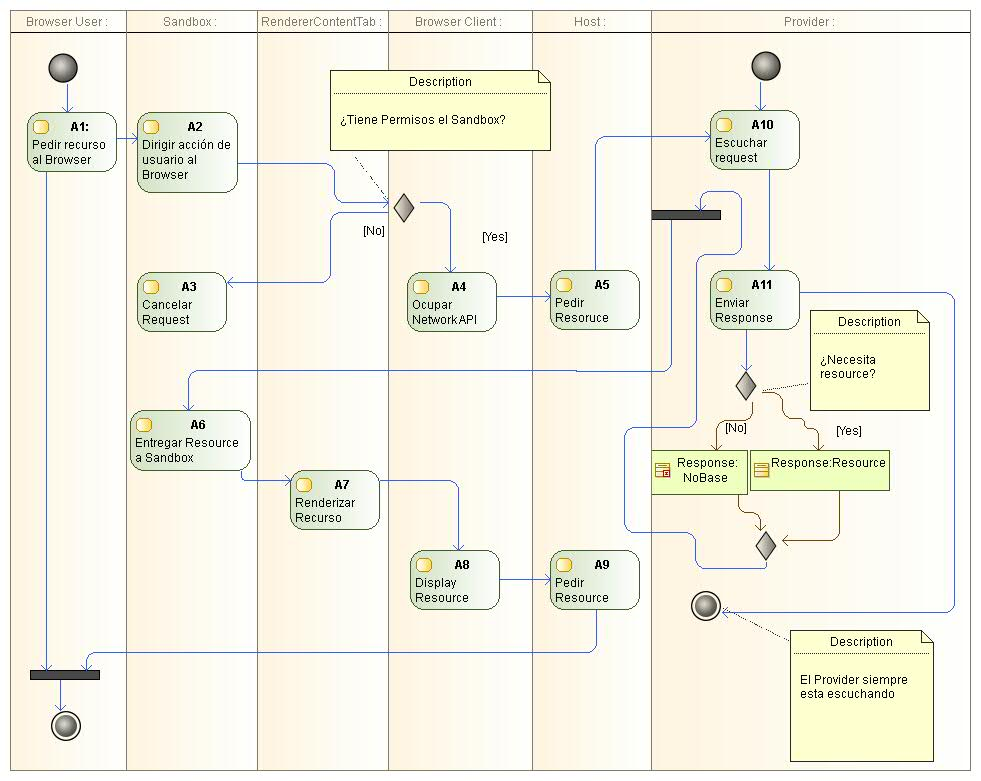
\includegraphics[scale=0.23]{figures/chap5/activityDiag_v3.jpg}
	    \caption{Diagrama de Actividad Compuesto para los casos de uso \textbf{Realizar Request} y \textbf{Recibir Request}.}
	    \label{fig:ActDiagr}
	\end{figure}
\end{frame}

\begin{frame}
	\frametitle{Diagrama de Clases para el patr\'on de Mal Uso.}
	\begin{figure}[h]
	    \centering
	    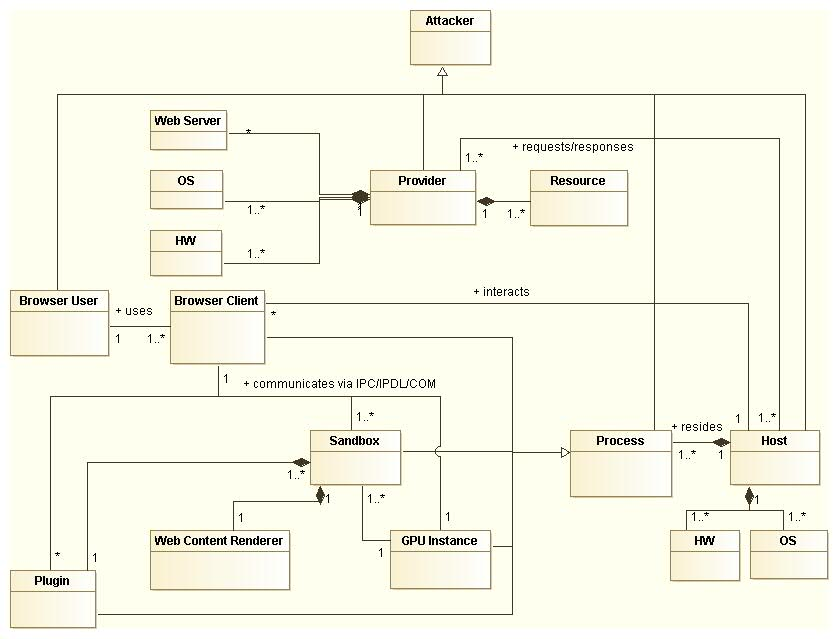
\includegraphics[scale=0.3]{figures/chap5/patronMisuse_v2.jpg}
	    \caption{Diagrama de Clases para el patr\'on de Misuse.}
	    \label{fig:BIMisuse}
	\end{figure}
\end{frame}

\begin{frame}
	\frametitle{Diagrama de Clases para el patr\'on de Mal Uso.}
	\begin{figure}[h]
        \centering
        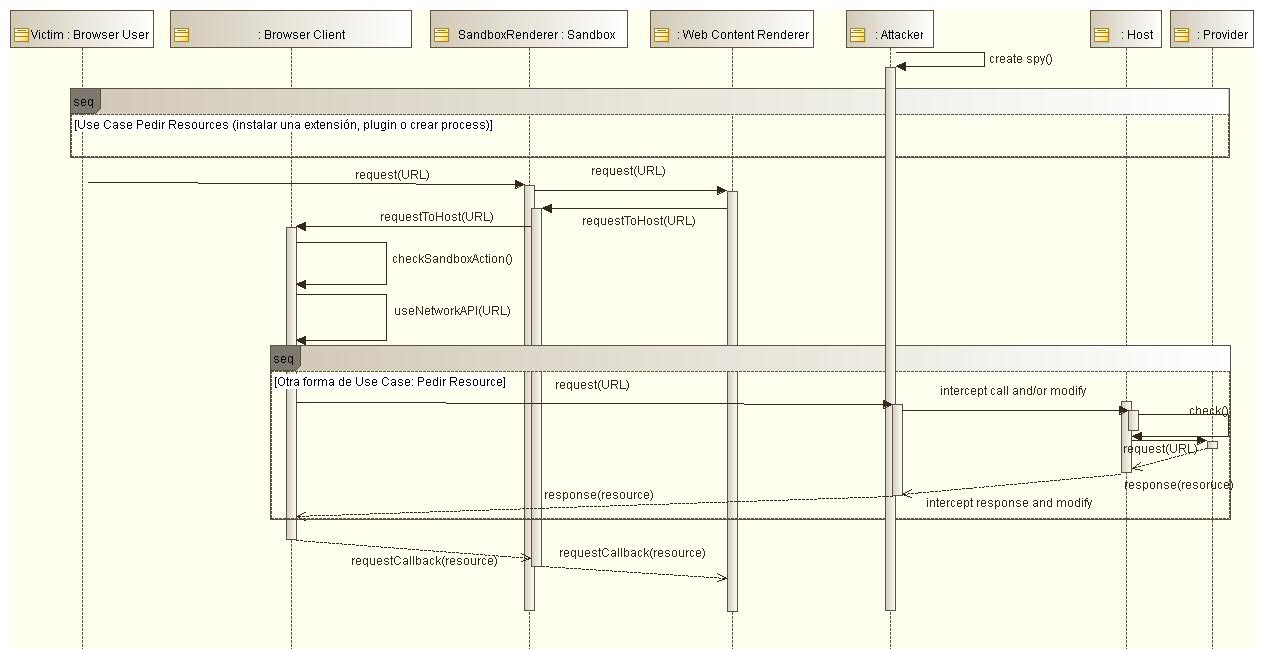
\includegraphics[scale=0.32]{figures/chap5/patronMisuseSeq_v2.jpg}
        \caption{Diagrama de Secuencia para el Mal uso: Modificaci\'on de tr\'afico en el \textit{Web Browser}.}
        \label{fig:SeqMisuse}
    \end{figure}
\end{frame}

\section{Conclusiones}
\begin{frame}
	\frametitle{Conclusiones}
	\begin{block}<1->{}
		Un navegador Web pareciera ser un Software de mediana complejidad: pero éste permite realizar una variadad de vectores de ataque, tanto en un usuario usándolo como en el sistema con el que 
	interactúa.
	\end{block}
\end{frame}

\begin{frame}
	\frametitle{Contribuciones}	
	\begin{itemize}
		\item<1-> Base Conceptual: términos de seguridad relacionados al navegador Web.
		\item<2-> Construcción del primer Patrón Arquitectural sobre la infraestructura del Web Browser.
		\item<3-> Una parte de la Arquitectura de Referencia ha sido construída, a través de la abstracción del Patrón Browser Infrastructure.
		\item<4-> Stakeholders y Casos de Uso más importantes
		\item<5-> Patrones de Mal Uso.
	\end{itemize}
\end{frame}

\begin{frame}
	\frametitle{Resumen}	
	\begin{itemize}
		\item<1-> Una śintesis y abstracción de la información correspondiente a los Web Browsers, para generar un lenguaje de comunicación de los conceptos. El uso de patrones permite ayudar a un conjunto de personas a unificar conceptos, así como también puede ser guía en futuros desarrollos.
		\item<2-> El trabajo propuesto permite comprender mejor, por medio de la Arquitectura de Referencia parcialmente construída, tanto componentes como amenazas existentes. Además como no está sujeto a implementaciones específicas, es posible generalizar ciertos resultados en otros Browsers.
		\item<3-> Comunicar en primera instancia, los conceptos de seguridad básicos para un mejor entendimiento de los subsistemas que interactuan en la Internet. Los patrones de Mal Uso permiten condensar la información y transmitirla, de forma ordenada y descriptiva.
		\item<4-> Entregar el conocimiento básico de los componentes e interacciones entre el Web Browser y un proveedor de recursos externo; así como también de las amenazas que existen
	\end{itemize}
\end{frame}

\begin{frame}
	\frametitle{¿Preguntas?}
	¡Muchas Gracias!	
\end{frame}

\bibliography{refTodas}
\bibliographystyle{IEEEtran}

\end{document}

